\section{Stato dell'Arte}
\label{sec:stato-arte}
In questa sezione verrà descritto lo stato dell'arte dei modelli \textit{agent-based} di evacuazione da tsunami, senza focalizzarsi sui modelli di inondazione.
Successivamente alcuni lavori verranno approfonditi nelle sottosezioni seguenti, in particolare modelli \textit{network-based} con scenari multimodali.

I primi modelli di evacuazione da tsunami sono stati basati sui modelli \textit{network-based} utilizzati per l'evacuazione da altri disastri come
uragani, incendi e inondazioni \parencite{usuzawa1997development, imamura2001development}.

Uno dei primi aspetti che è stato preso in considerazione è il comportamento umano,
in particolare le reazioni dei residenti all'arrivo dello tsunami
e il tempo che ci mettono per iniziare a evacuare.

Queste informazioni sono state raccolte tramite dei questionari rivolti ai residenti
e usate per stimare i tempi di partenza dell'evacuazione \parencite{imamura2001development, saito2004simulation}.

Questi primi modelli \textit{network-based} hanno usato come regola di \textit{path finding}
proseguire verso il nodo con altitudine maggiore.
Successivamente si è passati a usare il percorso
più breve \parencite{katada2004disaster} e altre strategie di routing basate sull'apprendimento 
come Nash equilibrium e system optimal \parencite{lammel2009towards}.

Un altro aspetto importante per l'evacuazione è la conoscenza dell'ambiente da parte degli agenti.
Alcuni lavori hanno distinto gli agenti in base alla loro conoscenza e
studiato gli effetti di diverse proporzioni tra categorie di agenti.
\textcite{nguyen2012simulation} hanno definito \textit{fox agent} un pedone ben informato che segue i segnali
stradali fino a un rifugio e \textit{sheep agent} un pedone che non sa
come comportarsi e quindi segue i \textit{fox agent} o si muove casualmente.
\textcite{takabatake2017simulated} invece hanno distinto gli agenti in residenti e visitatori.
I residenti sono agenti che conoscono il percorso più breve per evacuare, mentre i visitatori
seguono gli altri scegliendo la strada con più individui o si muovono verso una zona più elevata.

Con l'aumento della potenza di calcolo è stato possibile passare da modelli \textit{network-based} a modelli \textit{grid-based} e ibridi.
Inoltre è stato possibile usare una quantità di dati maggiore e sfruttare il calcolo parallelo \parencite{wijerathne2013hpc, makinoshima2018enhancing}.

\textcite{wijerathne2013hpc} hanno proposto un modello \textit{grid-based} che utilizza un sistema di navigazione basato
sulla visione. Gli agenti si muovono verso un luogo sicuro ben visibile scegliendo la strada con una maggiore distanza di visione.
%
Anche in questo lavoro vengono distinti visitatori, che si affidano alla visione, e non-visitatori, che hanno conoscenza di un'area
limita al di fuori della quale vengono considerati visitatori.

In molti modelli vengono considerati esclusivamente solo pedoni, ma alcuni lavori hanno analizzato l'aggiunta della presenza di auto e altri veicoli,
e si concentrano nella gestione delle interazioni tra i diversi tipi di agenti \parencite{goto2012tsunami, wang2016agent, wang2021novel}.

\subsection{L\"ammel, Rieser et al. (2010)}
Questo lavoro utilizza un modello \textit{network-based} per simulare un'evacuzione in larga scala di 450,000 pedoni.

All'inizio della simulazione tutti gli agenti siano nelle loro abitazioni 
e inizino ad evacuare dopo un certo tempo di partenza individuale.

I pedoni evacuano seguendo il percorso più breve e per alcuni di essi viene effettuato un \textit{re-planning} del percorso tramite Nash equilibrium,
considerando i tempi di attraversamento sulle strade.

La simulazione del traffico è implementata con un sistema a code dove ad ogni link viene assegnata una coda FIFO, 
limitata nel flusso in uscita \textit{flow capacity} e nella capacità di pedoni al suo interno \textit{storage capacity}.

La velocità viene aggiornata tramite la relazione $v = \min[v_{max}, FC / D]$, dove $v$ la velocità,
$V_{max}$ la velocità massima, $D$ la densità e $FC$ è la \textit{flow capacity} (Fig. \ref{fig:queue-model}).
%
Inoltre è stata considerata una velocità massima di 1.66 m/s per considerare il
flusso dei pedoni in caso di emergenza.

\begin{figure}[ht]
    \centering
    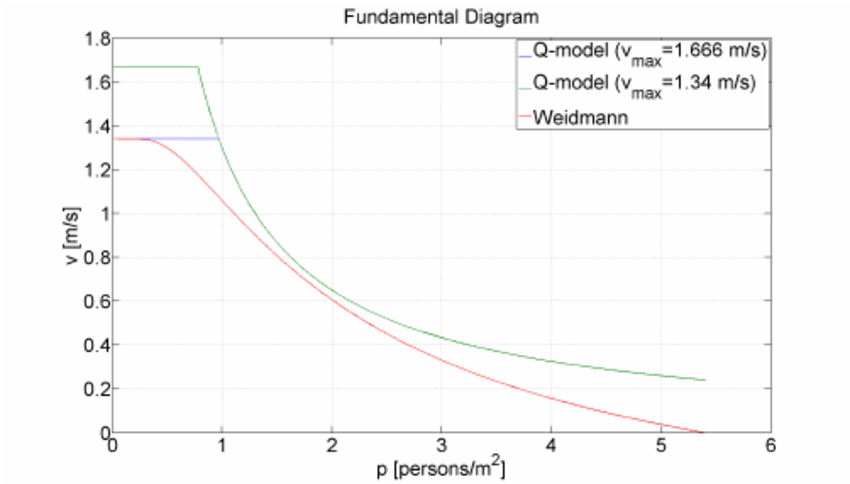
\includegraphics[width=0.6\textwidth]{images/queue-model.png}
    \caption{Diagramma fondamentale del modello a code confrontato con quello di \textcite{weidmann1993transporttechnik}.}
    \label{fig:queue-model}
\end{figure}

\subsection{Goto et al. (2012)}
In questo lavoro sono stati modellati diversi tipi di agenti raggruppati in famglie: pedoni lenti, pedoni normali, motociclisti e occupanti di un'auto.
Ogni agente rappresenta una famiglia che è formata da un numero diverso di individui in base al tipo di agente.
%
La velocità dei pedoni e dei motocicli viene aggiornata in base alla densità
e sono state gestite le interazioni tra i diversi agenti all'interno di una corsia stradale e i passaggi da una corsia all'altra.

La popolazione considerata è composta da oltre 20,000 individui ed è stato assunto che tutti si trovino a casa all'inizio dell'evacuazione.
%
Gli agenti evacuano seguendo il percorso più breve verso il rifugio più vicino. Nel caso di traffico elevato le auto possono aspettare o seguire il secondo percoso più breve.
Alcuni dei rifugi prevedono una capacità limita, che nel caso venga raggiunta la capacità massima gli agenti dovranno cambiare destinazione.

Un agente colpito dallo tsunami muore quando la profondità dello tsunami supera 1 m.

\begin{figure}[ht]
    \centering
    \begin{subfigure}{0.4\textwidth}
        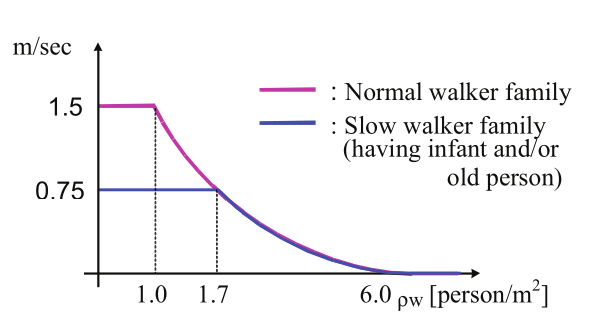
\includegraphics[width=\textwidth]{images/speed_GOTO.png}
        \caption{}
        \label{fig:goto-ped}
    \end{subfigure}
    \begin{subfigure}{0.4\textwidth}
        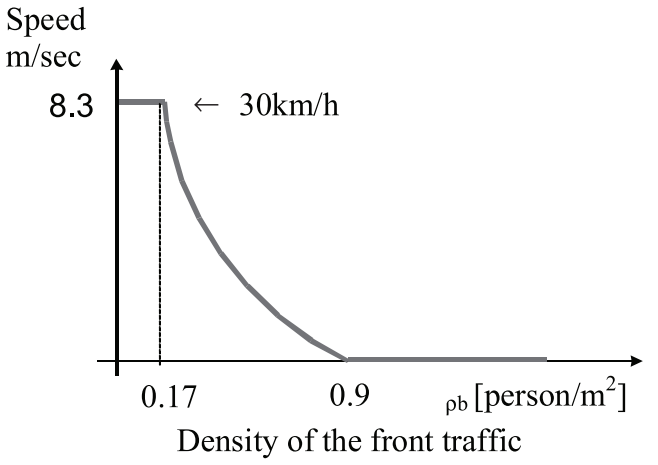
\includegraphics[width=\textwidth]{images/speed_GOTO_motocicli.png}
        \caption{}
        \label{fig:goto-moto}
    \end{subfigure}
    \begin{subfigure}{0.4\textwidth}
        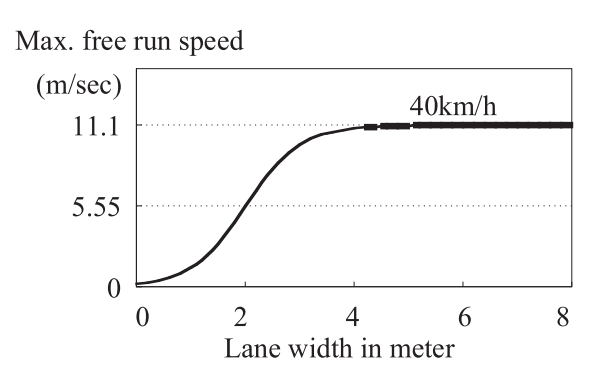
\includegraphics[width=\textwidth]{images/speed_GOTO_auto.png}
        \caption{}
        \label{fig:goto-auto}
    \end{subfigure}
    \caption{Relazione velocità-densità per i pedoni (a), per i motocicli (b), e relazione velocità-larghezza per le auto (c).}
    \label{fig:ankdasndk}
\end{figure}

I pedoni sono distinti in \textit{normal walkers}, con velocità massima di 1.5 m/s, e
\textit{slow walkers} (famiglie con disabili, anziani o bambini), con velocità massima di 0.75 m/s.
%
La velocità viene aggiornata al variare della densità con un massimo di $6 p/m^2$ (Fig. \ref{fig:goto-ped}).

Per i motocicli è stata considerata una velocità massima di 30km/h e una densità massima di 0.9 $p/m^2$ (Fig. \ref{fig:goto-moto}).

Per pedoni e motocicli la densità viene calcolata tramite la seguente formula:
$\rho = n /(L \times W)$, dove $n$ è il numero di agenti nell'area di fronte all'agente $L \times W$, $L$ è la lunghezza di ricerca 
e $W$ la larghezza della strada.

Le auto in assenza di ostacoli si muovono per $L_{f} = V_{f} \times \Delta_{t} $, dove $L_{f}$ è la \textit{free run length},
$V_{f}$ la velocità massima e $\Delta_{t}$ il \textit{time step}.
La velocità cambia in base alla larghezza della strada e può raggiungere una velocità massima di 40 km/h (Fig. \ref{fig:goto-auto}).
Per le auto invece la densità è definita da $\rho = n /((W - W_{c}) x L_{f})$, dove $W_{c}$ è la larghezza di un auto.
In base alla densità l'auto si muoverà fino al prossimo ostacolo, oppure fino alla prossima auto se presente.

Nel calcolo della densità un auto viene considerata 10 volte un pedone, mentre un motociclo 2 volte un pedone.

\subsection{Takabatake et al. (2017)}
In questo lavoro è stato sviluppato un modello di evacuazione da tsunami che considera
21,238 pedoni distinti tra residenti e visitatori.

I residenti si assume che conoscano il percorso più breve
per il rifugio più vicino dal punto in cui si trovano all'inizio dell'evacuazione.
%
I visitatori invece seguono due regole adottando un approccio probabilistico:
\begin{itemize}
    \item “following other individuals”: ad ogni intersezione seguono la strada con più individui.
    \item “going to higher ground”: ad ogni intersezione scelgono la strada che porta a un altezza maggiore.
\end{itemize}

Sia i residenti che i visitatori vengono distinti in base all'età con una velocità massima di 1.19 m/s (Under 65) e 0.96 m/s (Over 65).
Basandosi sul lavoro di \textcite{older1968movement} hanno assunto una decrescità lineare della 
velocità da un livello di densità di 0.3 p/m² a uno di 3.0 p/m² (Fig. \ref{fig:speed-linear}).

\begin{figure}[ht]
    \centering
    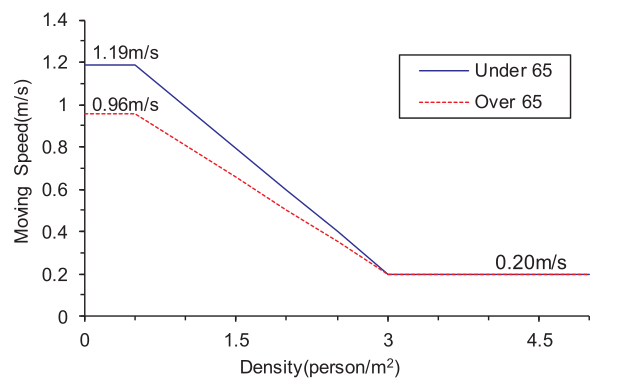
\includegraphics[width=0.7\textwidth]{images/speed_Linear.png}
    \caption{Relazione velocità-densità \textcite{takabatake2017simulated}}
    \label{fig:speed-linear}
\end{figure}

Per quanto riguarda i tempi di partenza sono stati usati due approcci sia per residenti che visitatori:
\begin{itemize}
    \item ``all-togheter'': gli agenti evacuano allo stesso tempo.
    \item ``delayed evacuation'': il tempo di partenza degli agenti viene assegnato secondo la distribuzione di Rayleigh.
\end{itemize}

I rifugi prevedono una capacità limitata. Quando un agente arriva in un rifugio già pieno si dovrà dirigere a un altro rifugio.
Per i visitatori viene applicato un delay di 30 secondi per chiedere informazioni sulla posizione del rifugio più vicino.

Il casualty model utilizzato considera che un agente muore quando l'altezza delle onde nella sua posizione supera i 0.3 m.


\subsection{Z. Wang e Jia (2021)}
In questo lavoro viene proposto un modello di evacuazione da tsunami multimodale e una valutazione dei rischi modellando l'incertezza
nei danni sismici nelle strade e in altri parametri del modello.

Sono state considerate diverse popolazioni al variare del numero di agenti: 5000 e 10,000,
che rappresentano la popolazione all'inizio dell'estate e 15,000 rappresenta il picco nella stagione estiva.

Gli agenti sono distinti in pedoni e auto ed evacuano verso il rifugio più vicino seguendo il percorso più breve.
Si assume che ogni auto contenga 4 agenti e che sia equivalente a 10 volte un pedone in spazio occupato.
Gli agenti per poter evacuare in auto dovranno prima raggiungere a piedi degli appositi parcheggi.

Il modello dei pedoni considera una velocità distribuita secondo una normale $\mathcal{N}(\mu_p,\sigma_p)$ troncata tra 0.75 m/s e 3.83 m/s e
con $\mu_p \sim \mathcal{U}(1.4, 2)$ e $\sigma_p \sim \mathcal{U}(0.1, 0.6)$.
Inoltre viene aggiornata in base alla densità di fronte all'agente con una \textit{search length} di 4m secondo l'andamento mostrato in figura \ref*{fig:dadknakdand}.

\begin{figure}[ht]
    \centering
    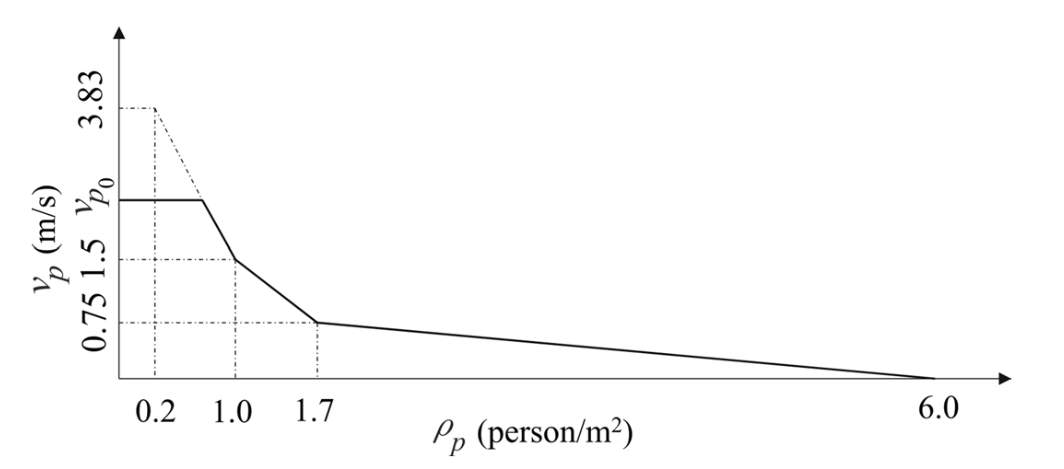
\includegraphics[width=0.7\textwidth]{images/speed_WANG.png}
    \caption{Relazione velocità-densità \textcite{wang2021novel} basato su un approssimazione del modello di \textcite{goto2012tsunami}}
    \label{fig:dadknakdand}
\end{figure}

Per le auto è stato utilizzato il modello di \textcite{greenshields1935study} che aggiorna la velocità in base alla densità di fronte lungo la \textit{free run length},
con una massima velocità di 40 km/h e una densità massima di 160 veh/km per i link senza restrizioni sul traffico date dai danni sismici, altrimenti 120 veh/km.

Per la gestione delle interazioni tra auto e pedoni vengono definite tre fasi di traffico in base al rapporto
tra il volume dei pedoni e delle auto: \textit{vehicle-dominated}, \textit{balanced} e \textit{pedestrian-dominated}.
Al variare della fase cambia la larghezza della strada occupabile sia per pedoni che per le auto.

Per i tempi di partenza viene utilizzata la distribuzione di Rayleigh dove i parametri
invece di essere fissati seguono delle apposite distribuzioni uniformi.

Rispetto ad altri lavori che utilizzano un livello di profondità fissa per determinare la morte degli agenti, in questo lavoro
viene considerato che la profondità sia distribuita uniformemente in [0.5, 3]. 
